\documentclass[aps,prb,reprint,groupedaddress]{revtex4-2}

\bibliographystyle{apsrev4-2}

\usepackage{physics}
\usepackage{bm}
\usepackage{amsfonts}
\usepackage{amssymb}
\usepackage{graphicx}
\usepackage{hyperref}
\hypersetup{colorlinks=true, citecolor=blue, urlcolor=blue, linkcolor=blue}

\begin{document}

\title{Rotating Chiral p-Wave Superfluid Under Annular Confinement}
\author{Junguang He}
\affiliation{Department of Physics, Northwestern University, Evanston, Illinois 60208, USA}
\author{Wei-Ting Lin}
\author{J. A. Sauls}
\email{sauls@lsu.edu}
\affiliation{Hearne Institute of Theoretical Physics, Louisiana State University, Baton Rouge, LA 70808, USA}
\date{August 17, 2025}

\begin{abstract}
    Persistent mass currents of a chiral p-wave superfluid confined in a toroidal annulus
    stabilize new equilibrium states. We present theoretical calculations of the
    corresponding phase diagram, the internal structure of the superfluid order parameter,
    and the angular momentum based on the Ginzburg-Landau free energy functional for
    $^3$He. For sufficiently small persistent current the angular momentum of the chiral
    phase is quantized in integer units given by the winding number of the global phase.
    These low-flow states can be stabilized by rotating the annulus at certain critical
    angular velocities. As the winding number is increased an asymmetry between the edge
    currents on the inner and outer radius develops, and at the critical value of the
    persistent current the superfluid undergoes a transition to a spatially inhomogeneous
    axial domain wall phase. We show that this phase is energetically favored at
    sufficiently large persistent current, with both the edge and domain wall currents
    counter-propagating relative to the bulk supercurrent. The axial domain wall state
    is also metastable down to zero bulk flow and exhibits a significantly increased
    angular momentum compared with the stable chiral ground state. This anomaly in the
    angular momentum is a direct signature of the axial domain wall phase of the
    superfluid condensate.
\end{abstract}

\maketitle

\section{Introduction}

Superfluid $^3$He is a spin-triplet, p-wave BCS condensate\cite{vollhardt13}.
The A phase of $^3$He is first proposed by Anderson and Morel\cite{Anderson61},
and it is a chiral p-wave superfluid of which the order parameter can be
represented by the 2$\times$2 spin matrix
$\Delta(\vb{p})=\vu{d}\vdot(i\va{\sigma}\sigma_y)\Delta(\vu{p}_m+i\vu{p}_n)$.
The orbital angular momentum of the Cooper pair is $+\hbar$ along the chiral
axis $\vu{l}=\vu{m}\cp\vu{n}$, and the Cooper pair spin has zero projection
along $\vu{d}$. Besides the A phase, which is one of the only two stable states
in bulk superfluid $^3$He, another one is the B phase which is fully gapped,
isotropic and has zero total angular momentum $J=0$.

Although there are only two stable states in bulk superfluid $^3$He, different
phases has been proposed theoretically under different geometric confinements.
Starting with translational invariant bulk B phase in thick films, crystalline
order is found in superfluid $^3$He confined in thin films with thicknesses
$9\xi(T)\approx D_{c_2}(T)<D<D_{c_1}(T)\approx13\xi(T)$\cite{vorontsov07},
where the order parameter breaks translational symmetry in plane of the film.
At $D_{c_2}$, the superfluid experience a first-order transition to the A phase
where the order parameter only has non-zero in-plane components, and $\vu{d}$
is locked perpendicular to the surface of the film. If we further confine in
the laterally direction, once again a pair density wave(PDW) phase which breaks
the translational invariance along the channel is found to be stable between
$9\xi_0\approx D_{c_2}<D<D_{c_1}\approx16\xi_0$\cite{Wu18}. For $^3$He confined
in nano channels, Stripe order is found in nano channels with radius $R<12\mu$m
at 0 bar\cite{Aoyama14}, and spontaneous helical order are found in channels with
$R=100$nm\cite{Wiman15,Wiman18}, which has NMR signatures as their `fingerprint'.

Experiments have been done to observe these different phases of superfluid $^3$He.
For thin films, the A and B phases are observed\cite{levitin10,Levitin13,zhelev17},
but the stripe phase has not been observed. However, evidence of a more complex
spatially modulated	phase is observed\cite{levitin19,shook20}.

\begin{figure}\label{AnnulusFig}
    \centering
    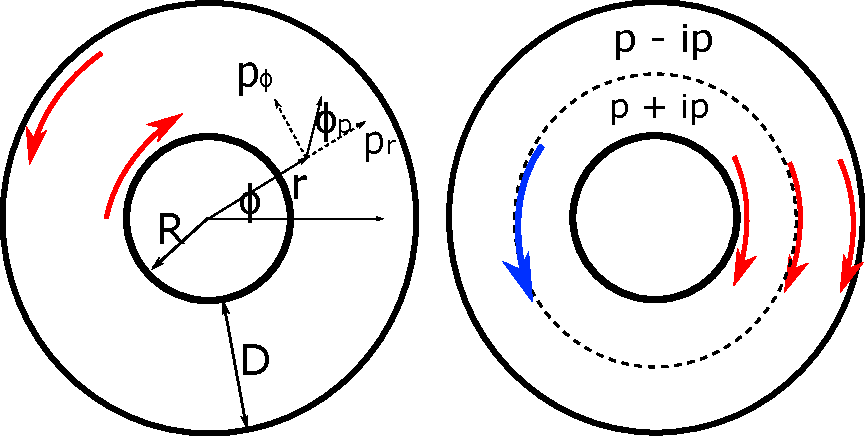
\includegraphics[width=8cm]{CylindricalBasis.pdf}
    \caption{The left panel shows a chiral p-wave superfluid confined in an
        annulus with inner radius $R$ and width $D$. The right panel is domain
        wall state where the red arrows are the edge/domain wall currents, and
        the blue arrow is the bulk flow.}
\end{figure}

The ground state angular momentum of chiral p-wave superfluid $^3$He-A at $T=0$
in a cylindrical thin film with radius much larger than the correlation length
$R\gg\xi_\Delta=\hbar v_f/2\Delta$ is $L_0=N\hbar/2$, where $N$ is the total
number of fermions and the ground state angular momentum can be interpreted as
$N/2$ Cooper pairs each with angular momentum $\hbar$\cite{mcclure79}. In
quasiclassical theory, the temperature dependence of the angular momentum is
the effective Yoshida function, $L=\pm L_0\mathcal{Y}(T)$\cite{Sauls11},
which near $T_c$ reduces to
\begin{align}
    \mathcal{Y}(T)\approx\left(\frac{\eta_0(T)}{T_c}\right)^2
    \frac{7\zeta(3)}{8\pi^2}\propto \left(1-\frac{T}{T_c}\right).
\end{align}
It has linear dependence on temperature because when $T\rightarrow T_c$, the bulk gap
$\eta_0\propto\sqrt{1-T/T_c}$. More generally, the angular momentum also depends on
the radius of the cylinder, especially when the
radius is of the order of the coherence length, the curvature of the confining wall
and the overlap of edge currents will alter the internal structure and hence
the angular momentum.

In this paper, we focus on the chiral p-wave superfluid under annular confinement,
along which there is a finite mass flow field. The edge states as well as domain
walls play important roles in determining the stable states of the superfluid.

In Sec.\ref{sec:GL} we introduce the GL theory of a 2D chiral p-wave superfluid
in cylindrical basis, and derived expression of the mass current density and
angular momentum of the system. In Sec.\ref{sec:ChiralCylinder} we calculate the
angular momentum suppression of the chiral state due to the curvature of the
confining wall, and we calculate the internal structure
of the $p=2$ doubly quantized vortex state in a cylinder, which is a hint for
the newly predicted axial domain wall state in an annulus discussed in Sec.\ref{sec:annulus},
where we also calculate the $v_s-D$ phase diagram near $T_c$. In
Sec.\ref{sec:AngularMomentum}, we discuss the different angular momentum of the
axial domain wall state compared with the chiral state, and the quantized angular momentum of the low
flow states with winding number $m>0$, which can be stabilized by rotating the annulus with
angular velocity $\Omega_m$. In Appendix \ref{appendix} we derive the weak-coupling
parameters of the chiral p-wave superfluid from the quasiclassical theory.

\section{Ginzburg-Landau Theory}\label{sec:GL}

For chiral p-wave superfluid $^3$He-A confined in an annular thin film in the $x-y$
plane, the chiral axis $\vu{l}\parallel\vu{z}$ is locked perpendicular to the surface.
The $\vu{d}$ is locked to be parallel to the direction of the chiral axis by nuclear
dipole energy, and the order parameter can be represented by the $2\times 2$ gap matrix,
\begin{align}
    \hat{\Delta}(\vb{r},\vu{p})=\vu{d}\vdot(i\vu{\sigma}\sigma_y)
    \bigg(\eta_i(\vb{r})\vu{p}_i+\eta_j(\vb{r}) \vu{p}_j\bigg),
\end{align}

In GL theory, the free energy functional that describes the chiral p-wave superfluid is
\begin{align}
    F[\bm{\eta}]=\int\dd[3]r\left(f_{\text{bulk}}+f_{\text{grad}}\right),
\end{align}
where the bulk free energy density is
\begin{align}
    f_{\text{bulk}}[\bm{\eta}] = \alpha\bm{\eta}\vdot\bm{\eta}^*
    +\beta_1(\bm{\eta}\vdot\bm{\eta}^*)^2
    +\beta_2|\bm{\eta}\vdot\bm{\eta}|^2,
\end{align}
with $\bm{\eta}=(\eta_i,\eta_j)$. In cartesian basis the bulk order parameter is
$(\eta_x^\text{bulk},\eta_y^\text{bulk})=\eta_0(1,\pm i)$ where
$|\bm\eta_{\text{bulk}}|=\sqrt{2}\eta_0=\sqrt{-\alpha/2\beta_1}$. The minimized bulk free
energy density is $f_\text{min}=-\alpha^2/4\beta_1$.
In cylindrical basis, the corresponding bulk order parameter is
$\eta_r(\phi)=\eta_0e^{\pm i\phi}$
and $\eta_\phi(\phi)=\pm i\eta_0e^{\pm i\phi}$, which gives
\begin{align}
    \hat{\Delta}(\phi,\vu{p})=\sigma_x\eta_0e^{\pm i\phi}(\vu{p}_r\pm i\vu{p}_\phi)
    \equiv\sigma_x\eta_0e^{\pm i(\phi+\phi_p)}.
\end{align}

In the Cartesian basis the gradient term which describes
the kinetic and bending energy of the system is
\begin{align}\label{GL}
    f_{\text{grad}}^{\text{Car}}[\bm{\eta}]= & \kappa_1(\partial_i\eta_j)(\partial_i\eta_j)^*
    +\kappa_2(\partial_i\eta_i)(\partial_j\eta_j)^*\nonumber                                    \\
                                             & +\kappa_3(\partial_i\eta_j)(\partial_j\eta_i)^*,
\end{align}
with $i,j=x, y$. We define $v_c = \hbar/M\xi$ where $M=2m$ is the mass of the
correlated pairs. The bulk critical flow field
is obtained by introducing a uniform
flow field $\vb{v}_s=\hbar\grad\theta/M$ where
$\eta(\vb{r})=|\eta|e^{iM\vb{v}_s\vdot \vb{r}/\hbar}$ such that
$f_{\text{bulk}}+f_{\text{grad}}=0$, which destroys the superfluidity.
% In weak-coupling limit the critical flow field for chiral phase
% is $v_c^\text{chiral} = v_c/\sqrt{2}$.

We can transform the free energy density into cylindrical basis by substituting in
$(\eta_r,\eta_\phi)^T=R^T(\phi)(\eta_x,\eta_y)^T$ and
$\va{\partial}=(\partial_r,\frac{1}{r}\partial_\phi)^T=R^T(\phi)(\partial_x,\partial_y)^T$,
where $R(\phi)$ is the 2-d rotation matrix\cite{Buchholtz77},

\begin{widetext}
    \begin{align}
        f_{\text{grad}}[\bm{\eta}]= & \kappa_1(\partial_i\eta_j)(\partial_i\eta_j)^*
        +\kappa_2(\partial_i\eta_i)(\partial_j\eta_j)^*
        +\kappa_3(\partial_i\eta_j)(\partial_j\eta_i)^*\nonumber                     \\
                                    & +\frac{2}{r}\Re{
            \kappa_1\left(\eta_r^*\frac{\partial_\phi}{r}\eta_\phi
            -\eta_\phi^*\frac{\partial_\phi}{r}\eta_r\right)
            +\kappa_2\eta_r^*\partial_j\eta_j
            +\kappa_3\left(\eta_r^*\frac{\partial_\phi}{r}\eta_\phi
        -\eta_\phi^*\partial_r\eta_\phi\right)}\label{fgrad}                         \\
                                    & +\frac{1}{r^2}\left[\kappa_1\eta^*_j\eta_j
            +(\kappa_2+\kappa_3)\eta_r^*\eta_r\right].\nonumber
    \end{align}
\end{widetext}

To determine the equilibrium stationary states, we derive the Euler-Lagrange
equations of the free energy functional by demanding the functional gradient
$\fdv*{F[\bm{\eta}]}{\bm{\eta}^*}=0$. This is the GL differential equation
\begin{widetext}
    \begin{align}\label{GL-cylin}
        \fdv{F}{\eta_k^*}=\alpha\eta_k
         & +2(\beta_1\eta_i\eta_i^*\eta_k
        +\beta_2\eta_i^2\eta_k^*)-\left(\kappa_1\partial_i^2\eta_k
        +\kappa_2\partial_k\partial_i\eta_i
        +\kappa_3\partial_j\partial_k\eta_j\right)\nonumber              \\
         & -\frac{1}{r}\left[(2\kappa_1+\kappa_3)\frac{\partial_\phi}{r}
            \left(\eta_r\delta_{k\phi}-\eta_\phi\delta_{kr}\right)+\kappa_1\partial_r\eta_k
            +(\kappa_2+\kappa_3)\partial_k\eta_r\right]
        +\frac{1}{r^2}[\kappa_1\eta_k+(\kappa_2+\kappa_3)\eta_r\delta_{kr}]
        =0.
    \end{align}
\end{widetext}
The first line of Eq.(\ref{fgrad}) and Eq.(\ref{GL-cylin}) are of the same form
as the Cartesian basis, and the other lines are additional terms in the cylindrical
basis. We can also derive Eq.(\ref{GL-cylin}) by transforming the Cartesian-basis
GL equation into cylindrical basis.

The boundary condition for maximal pair breaking is just both components vanishes
at the edge, while for minimal pair breaking, the boundary condition is modified
by the presence of curvature. For the Euler-Lagrange surface term to vanish,
we have\cite{Buchholtz77}
\begin{align}
    \eta_r=0,\qq{} \partial_r\eta_\phi=\frac{\eta_\phi}{r},
\end{align}
which returns to the boundary condition in Cartesian basis when $r\rightarrow\infty$.

The superfluid mass current density or the momentum density in the cylindrical basis is
\begin{align}\label{j}
    \vb{j}_k=\frac{2M}{\hbar}\bigg[\Im{\kappa_1\eta_j^*\partial_k\eta_j+\kappa_2\eta_k^*\partial_j\eta_j+\kappa_3\eta_j^*\partial_j\eta_k}\nonumber \\
        +\Im{(2\kappa_1+\kappa_2+\kappa_3)\delta_{k\phi}\eta_\phi^*\eta_r/r}\bigg],
\end{align}
In weak-coupling limit,
where $\beta_1=2\beta_2$ and $\kappa_1=\kappa_2=\kappa_3$, the angular momentum
density $l_z=rj_\phi$ becomes
\begin{align}\label{l_density}
    l_z=\frac{2M\kappa_1}{\hbar}\bigg[\Im{3\eta_\phi^*\partial_\phi\eta_\phi+\eta_r^*\partial_\phi\eta_r+4\eta_\phi^*\eta_r}\nonumber \\
        +\Im{r\eta_\phi^*\partial_r\eta_r+r\eta_r^*\partial_r\eta_\phi}\bigg].
\end{align}
There are two contributions to the angular momentum density Eq.(\ref{l_density}).
The first two terms are associated with $\partial_\phi$, which
generally corresponds to the azimuthal direction phase gradient, i.e. the bulk flow,
while the last two terms are associated with $\partial_r$, which corresponds to the
order parameter distortion, i.e. the mass current confined to the edges or domain
walls.

The total angular momentum can be calculated by a volume integral of the
angular momentum density. In general, for the cylindrical and annular
geometry we are concerned in this chapter,
we can define the total angular momentum as
$L[\bm{\eta}] = \int\dd[3]rl_z \equiv \frac{2M\kappa_1V\eta_0^2}{\hbar} \mathcal{L}[\bm{\eta}] $
where
\begin{align}\label{total_L}
    \mathcal{L}[\bm{\eta}] =
     & \ev{3\eta_\phi^*\partial_\phi\eta_\phi
        +\eta_r^*\partial_\phi\eta_r
    +4\eta_\phi^*\eta_r}_V\nonumber           \\
     & +\ev{r\eta_\phi^*\partial_r\eta_r
        +r\eta_r^*\partial_r\eta_\phi}_V,
\end{align}
The angle brackets above denotes the volume average,
\begin{align}
    \ev{...}_V=\int\frac{\dd[3]r}{V}\frac{\Im{...}}{\eta_0^2},
\end{align}
Note that we can define $j_c\equiv|f_\text{min}|/v_c$ and $l_c\equiv j_c\xi$, then we have
$L[\bm{\eta}] = 2l_c V \mathcal{L}[\bm{\eta}]$.
The functional $\mathcal{L}[\bm{\eta}]$
is basically the average of the angular momentum density,
and it reflects the modification to the total angular momentum
due to confinement and bulk flow of the system.

We can write everything into dimensionless form using the coherence length
$\xi^2=\kappa_1/|\alpha|$, and the bulk gap $\eta_0$.

\section{Stationary States in a Cylinder}\label{sec:ChiralCylinder}

\begin{figure}
    \centering
    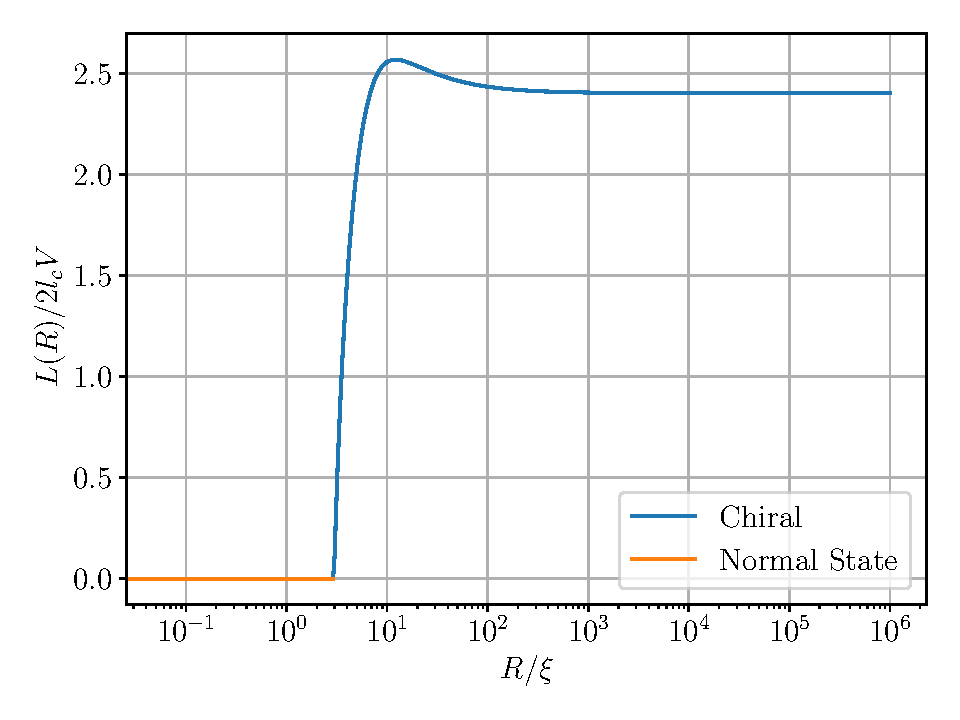
\includegraphics[width=8cm]{L_r.pdf}
    \caption{Ground state angular momentum of chiral p-wave superfluid
        in a cylinder as a function of radius $R$ near $T_c$.}
    \label{fig:L_r_cylinder}
\end{figure}

For superfluid $^3$He-A confined in a cylindrical thin film,
the order parameter should be single-valued everywhere in the cylinder.
When the system has axial symmetry, i.e. the radial and azimuthal directions are decoupled,
we can Fourier transform the azimuthal angle dependence using
the winding number $n$,
\begin{align}
    \eta_j(r,\phi)=\sum_{n=-\infty}^{\infty}\eta_j^{(n)}(r)e^{in\phi}.
\end{align}

We further assume the order parameter to be rotationally invariant
up to a global phase factor, i.e. $\eta_j(r,\phi)=\eta_j^{(n)}(r)e^{in\phi}$.
In this case, we can substitute $\partial_\phi\rightarrow in$
in the free energy functional and the GL equations.
In this case, the total angular momentum of the superfluid confined in the cylinder
depends on the radius $R$, i.e. $L = 2l_c V \mathcal{L}(R)$.
When we reduce the radius of the cylinder, the curvature of the confining wall
and the overlap of the edge current will start to modify the internal structure
and the angular momentum. We neglect any possible axial-symmetry breaking states
with this effectively 1-d model. When the radius becomes smaller, as shown in
Fig. \ref{fig:L_r_cylinder}, the geometric factor $\mathcal{L}(R)$ first slightly
increases and then decreases due to strong pair breaking. The slight increase is
due to a larger portion of edge state area when we reduce the radius $R$, since
the ground state angular momentum mostly comes from the edge current. At a smaller
radius than the critical radius $R_c$, the edge current becomes so significant that
it destroys the superfluid states and there will be no intrinsic angular momentum.

\begin{figure}
    \centering
    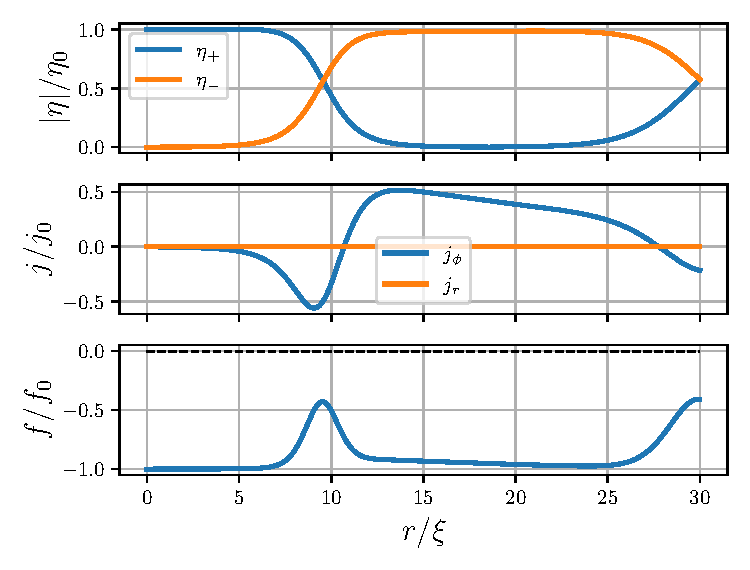
\includegraphics[width=8cm]{-p+ip_m=2.pdf}
    \caption{Order parameter, mass current density, and free energy
        density profile of the doubly quantized vortex state with local
        winding number $m=0$ and global winding numeber $p=2$.}
    \label{2vortex}
\end{figure}

Other possible cylindrically symmetric states up to
a global phase factor are the vortex states or a normal
metallic inclusion. We can define a new basis
$\eta_\pm$ where
\begin{align}
    \eta_r    & \equiv\eta_+e^{i\phi}+\eta_-e^{-i\phi},     \\
    \eta_\phi & \equiv i(\eta_+e^{i\phi}-\eta_-e^{-i\phi}),
\end{align}
and the winding number of the $\eta_\pm$ components are off by 2, i.e.
\begin{align}
    \eta_+(r,\phi)=\eta_+^{(m)}(r)e^{im\phi}, \\
    \eta_-(r,\phi)=\eta_-^{(p)}(r)e^{ip\phi},
\end{align}
where $n=m+1=p-1$. This relation comes out naturally as a result of monochromatic
phase winding of the order parameter, and can also be interpreted via a total angular
momentum conservation perspective, see reference\cite{sauls09}.

For the doubly-quantized vortex in a cylinder with radius $R=30\lambda$
shown in Fig. \ref{2vortex}, the local order
parameter $\eta_+$ with phase winding $m=0$ and global order parameter $\eta_-$ with
phase winding $p=2$ are separated by a lateral type domain wall at the radius of about
$10\xi$. The lateral component of the order parameter $\eta_\phi$ changes sign
across the domain wall. Other types of doubly-quantized($p=-2$) and
singly-quantized($p=\pm 1$) vortices and the normal metallic inclusion($p=0$) have a
local phase winding $m\neq 0$ and the order parameter $\eta_j(r=0)=0$ vanishes
at the vortex core\cite{sauls09}.
The order parameter of this particular doubly-quantized vortex
with $p=2$ and $m=0$ does not vanish at the vortex core, which provides a hint for
possible internal structure in an annulus, where the lateral type domain wall also
separates the inner and outer half of the annulus into two domains with opposite
chirality.

\section{Competing phases in Annular geometry}\label{sec:annulus}

\begin{figure}
    \centering
    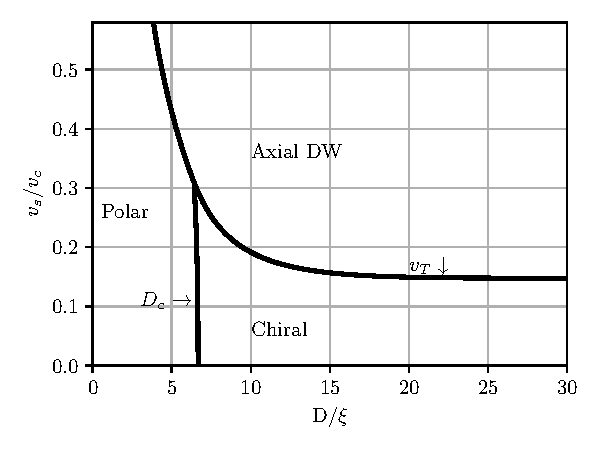
\includegraphics[width=8cm]{phase_diagram.pdf}
    \caption{The $v_s-D$ Phase diagram of a annularly confined chiral p-wave superfluid with inner radius $R\gg\xi$.}
    \label{PhaseDiagram}
\end{figure}

We consider an annulus with inner radius $R\gg\xi$ and annulus width
$D\sim\xi$(Fig. \ref{AnnulusFig}). For simplicity we still assume rotational symmetry
up to a global phase factor, i.e. $\bm{\eta}(r,\phi)=\bm{\eta}^{(n)}(r)e ^{in\phi}$.
This assumption neglect any possible axial symmetry breaking states, like vortex
states, but in a narrow annulus it is generally difficult to generate vortices.
Since we have $R\gg\xi$, the curvature of the confining wall can be neglected,
and the annulus can be approximated as a straight channel. The nonzero phase
winding may correspond to a uniform persistent current flow in
the annulus, with the velocity field at the inner radius as,
\begin{align}\label{vs}
    \vb{v}_s=\frac{\hbar}{M}\grad\theta=n\frac{\hbar}{MR}\vu{\phi}.
\end{align}
The winding number $n=\frac{R}{\xi}\frac{v_s}{v_c}$ can be easily of the order of
$R/\xi\gg1$, so instead we use the flow velocity $v_s$ of the superfluid to describe
different states.

The polar phase is the stable state when the annulus is narrow
$D<D_c\sim 7\xi$(Fig. \ref{PhaseDiagram}). The
radial component $\eta_r$ is suppressed to zero everywhere in the annulus.
The azimuthal component $\eta_\phi$ becomes homogeneous, and its amplitude decreases
as the flow field $v_s$ increases. The critical flow field of the polar phase is
$v_c^\text{polar}=v_c/\sqrt{3}$, where superfluidity is destroyed.

\begin{figure}
    \centering
    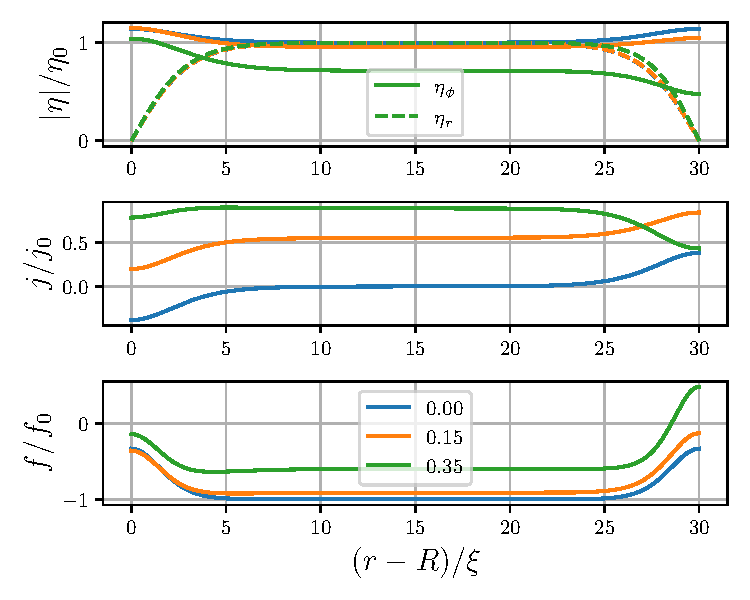
\includegraphics[width=8cm]{chiral.pdf}
    \caption{Order parameter, mass current density, and free energy density
        profile of the chiral state with bulk flow $v_s/v_c=0, 0.15, 0.35$.}
    \label{chiralOP}
\end{figure}

When $D>D_c$ and the flow field is small $v_s<v_T\sim 0.15v_c$, the
chiral phase is the stable state(Fig. \ref{PhaseDiagram}).
For the minimal pair-breaking boundary condition
the radial component, $\eta_r$, which is perpendicular to the boundary, vanishes at the inner
and outer radius, while the azimuthal component $\eta_\phi$ is slightly enhanced(Fig. \ref{chiralOP}).
As we increase the flow field, the order parameter at the inner and outer radius
becomes asymmetric. For the case with positive chirality, i.e. $p_r+ip_\phi$, the order
parameter at the outer radius will be more suppressed than the inner radius because
the edge current is propagating in parallel to the bulk flow,
resulting in a larger local current density and stronger pair-breaking effect.
The local free energy density is also higher, which may be energetically
unfavorable under larger bulk flow. Indeed if we further increase the flow field beyond
a critical value($\sim 0.35v_c$), the chiral state becomes unstable and
we do not converge to a chiral solution to the GL equation(Fig. \ref{L_F_v}).

\begin{figure}
    \centering
    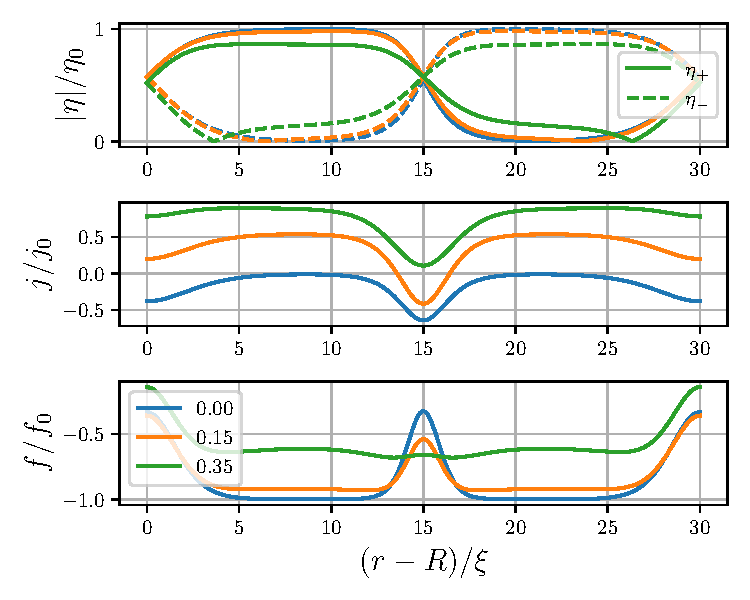
\includegraphics[width=8cm]{mix.pdf}
    \caption{Order parameter, mass current density, and free energy density
        profile of the domain wall state with bulk flow $v_s/v_c=0, 0.15, 0.35$.}
    \label{DWOP}
\end{figure}

The phase diagram of a chiral p-wave superfluid confined in an annulus with finite
bulk flow is shown in Fig. \ref{PhaseDiagram}. For the chiral to axial DW phase
transition, there is a free energy competition between the domain wall and the edge
state at the outer radius(Fig. \ref{chiralOP},\ref{DWOP}). Since the outer
edge current of the chiral phase propagates parallel to the bulk flow, flipping the
direction of the outer edge current by introducing a negative-chirality domain in
the outer half of the annulus will reduce the local current density and thus the free energy
density. But when the bulk flow is small $v_s<v_T$, the back flow introduced by the
lateral DW will increase the local current density and free energy density at the
middle of the annulus, resulting in an increased free energy. When the bulk
flow is large $v_s>v_T$, the counter propagating domain wall current reduces the
local current density and free energy density at the middle of the annulus, making
the axial DW phase energetically favorable. This free energy competition happens
between the domain wall and the edge state, and is irrelevant to the width of the
bulk regions of the two domains, so we expect that the transition flow velocity
between the chiral and axial domain wall phase will saturate to a constant value of
$v_T\approx0.15v_c$ as $D$ increases. As the annulus becomes wider, it is also
easier to generate vortices under large bulk flow, but vortex states are neglected
in our 1-d model. Possible rotational symmetry breaking states(similar to
the PDW state in a straight channel) are also neglected.

\section{Angular Momentum Anomaly}\label{sec:AngularMomentum}

For an annulus with $R\gg D=30\xi$, when $v_s$ is small, as we increase the flow field,
the angular momentum will increase linearly(Fig. \ref{L_F_v}). We can see this in
the London limit where we assume $\bm{\eta}(\phi)=\eta_0(1,i)e^{in\phi}$,
and $n=\frac{R}{\xi}\frac{v_s}{v_c}$ as in Eq.(\ref{vs}).
Substitute in Eq.(\ref{total_L}), and we have
\begin{align}
    \mathcal{L}(v_s) = 4 \frac{R}{\xi} \frac{v_s}{v_c}.
\end{align}
As the flow field becomes larger, the order parameters become more suppressed and will
decelerate the increase and even decrease angular momentum. Hence the angular momentum
has a maximum value with respect to the bulk flow.

For the axial domain wall state, the angular momentum can experience a sign change as
the bulk flow increases(Fig. \ref{L_F_v}), since the angular momentum is negative
at $v_s=0$. For the phase transition from the chiral to axial DW state, the angular
momentum will have a sudden drop, since both edge currents and the domain wall current
propagates anti-parallel to the bulk flow, resulting in a smaller angular momentum.

For the ground state of chiral p-wave superfluid in an annulus at zero temperature and zero bulk flow,
assuming a constant-$\Delta$ model, the angular momentum is $L_0=N\hbar/2$ as long as
the inner radius and the width of the
annulus is large $R, D\gg\xi$. In this case the edge states are confined to the
boundary at the length scale $\xi$ and the edge current density is a delta function at
the inner and outer radius with amplitude $n\hbar/4$. The edge current density distribution
is
\begin{align}
    j(r) = \bigg[\delta(r-R-D) - \delta(r-R)\bigg] \frac{n}{4}\hbar,
\end{align}
where $n$ here is
the number density of the total fermions in the system\cite{Sauls11}. For finite temperatures,
we just multiply the mass current density $j(r,T) = j(r) \mathcal{Y}(T)$ and total angular
momentum $L_\pm(T) = \pm L_0\mathcal{Y}(T)$ by the temperature dependence.

The axial domain wall state is metastable at zero bulk flow $v_s=0$. With both edge currents
and the domain wall current propagating in the same direction, its angular momentum has a
larger amplitude compared with the chiral state. Numerical calculation shows that the amplitude
of domain wall current is larger than the edge current, which we denote as $\alpha n\hbar/4$.
The current distribution of the axial domain wall state at zero bulk flow is
\begin{align}
    j_\text{dw}(r) = -\bigg[ & \delta(r-R) + \delta(r-R-D)\nonumber                             \\
                             & +\alpha\delta\left(r-R-\frac{D}{2}\right)\bigg]\frac{n}{4}\hbar.
\end{align}
The total angular momentum is
\begin{align}
    L_{\text{dw}} & = \int rj_\text{dw}(r)\dd[3]r\nonumber         \\
                  & =L_-\frac{(2+\alpha)(w^2+w)+1+\alpha/4}{2w+1},
\end{align}
and we have
\begin{align}
    L_{\text{dw}}\xrightarrow{w\gg 1} L_-\left(1+\frac{\alpha}{2}\right)w,
\end{align}
where $w=R/D$ is the ratio of the inner radius to the annulus width. At zero bulk flow,
the angular momentum of the axial domain wall state can have a much larger angular momentum
than the chiral phase when $w\gg 1$.  Similar idea was proposed using rough surface to
eliminate one of the two counter-propagator edge current\cite{Sauls11}, but here we are
using the property of the internal current structure of the axial domain wall state
and do not need to manipulate the surface condition.
\begin{figure}
    \centering
    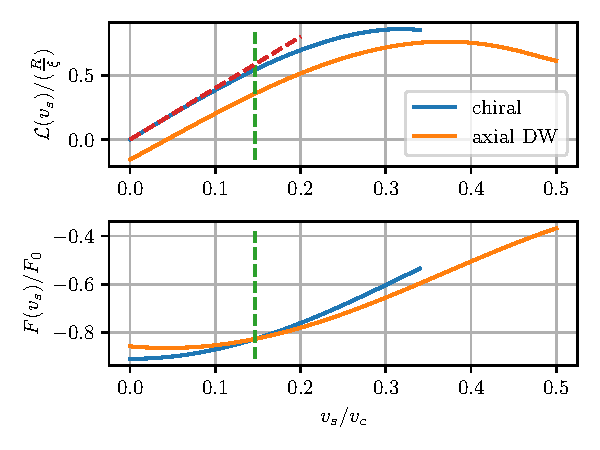
\includegraphics[width=8cm]{L_v.pdf}
    \caption{Angular momentum and free energy of the chiral and domain wall state
        of annularly confined chiral p-wave superfluid with inner radius $R\gg\xi$ and $D=30\xi$.}
    \label{L_F_v}
\end{figure}

For the low-flow states of the chiral phase in an annulus with $R,D\gg \xi$,
the flow field and the angular momentum are quantized in unit of the winding
number $m$. When $m$ is small, the flow is not large enough to greatly change
the radial direction gap profile. For the constant-gap model, we assume
\begin{align}
    \eta_r^{(m)}(R<r<R+D,\phi) & =\eta_0 e^{\pm i\phi} e^{im\phi},      \\
    \eta_r^{(m)}(r=R,\phi)     & =\eta_r(r=R+D,\phi)=0,                 \\
    \eta_\phi^{(m)}(r,\phi)    & =\pm i\eta_0 e^{\pm i\phi} e^{im\phi}.
\end{align}
By substituting the order parameter into Eq.(\ref{total_L}), we will get
$L_\pm(m)=(2m\pm 1)L_\pm(0)$, while self-consistent calculation gives
\begin{align}
    L_\pm(m)\approx(1.7m\pm 1)L_\pm(0),
\end{align}
where the $\pm$ corresponds to the time-reversed degenerate ground states,
i.e. $p_x+ip_y$ and $p_x-ip_y$. Here the angular momemtum of the time-reversed
states with $m=1$ has approximately a four times difference in magnitude,
i.e. $L_+(1)\approx 3.86L_-(1)$.

\begin{figure}
    \centering
    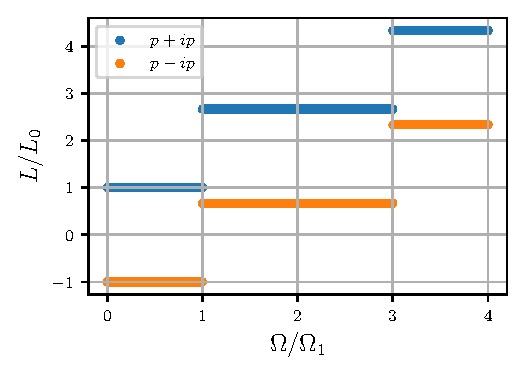
\includegraphics[width=8cm]{L_m.pdf}
    \caption{Quantized angular momentum of low-flow chiral states.}
    \label{L_m}
\end{figure}

We can stabilize these low-flow states by rotating the annulus at
certain angular velocities $\Omega_m$. Transform into the rotating frame
with angular velocity $\vb{\Omega}=\vu{z}\Omega$, and the free energy becomes
\begin{align}
    F' & =F-\vb{L}\vdot\vb{\Omega}.
\end{align}
The critical angular velocity $\Omega_m$ which increase
the winding number from $m-1$ to $m$ should
satisfy $F'(m,\Omega_m)=F'(m-1,\Omega_m)$, which gives
\begin{align}
    \Omega_m^\pm=\frac{F_\pm(m) - F_\pm(m-1)}{L_\pm(m) - L_\pm(m-1)}.
\end{align}
When the winding number $m$ is small, under certain approximations (Appendix \ref{appendix2}),
we have
\begin{align}
    \Omega_m^\pm \approx \frac{\hbar}{MR^2}\left[\left(m-\frac{1}{2}\right)
        \pm\left(\frac{2}{a}\ln(2)+b\right)\frac{\xi}{D}\right],
\end{align}

\section{Summary and Outlook}\label{sec:summary}

For the chiral p-wave superfluid confined in a cylinder,
the ground state angular momentum
$L = \frac{2M\kappa_1V\eta_0^2}{\hbar} \mathcal{L}(R)$ depends on the radius,
where $\mathcal{L}(R)$ measures the angular momentum with respect to a fix
number of particles. Starting from $R\gg\xi$ and decrease the radius, $\mathcal{L}(R)$
will first slightly increase due to a larger portion of the edge state area, and
then drops to zero due to significant pair-breaking effect by the strong
confinement(Fig. \ref{fig:L_r_cylinder}). We also reproduced various vortex states
originally predicted by quasiclassical theory, which inspires us of the newly
predicted axial domain wall phase of chiral p-wave superfluid confined in an annulus.

For the chiral p-wave superfluid confined in an annulus with inner radius
$R\gg\xi$ and a finite uniform flow field $v_s$, the $v_s-D$ phase
diagram(Fig. \ref{PhaseDiagram}) is calculated.
The axial domain wall phase is stabilized with $D>D_c\sim7\xi$ and $v_s>v_T\sim0.15v_c$.
The order parameter has an internal structure of an axial domain wall separating
the two time-reversed chiral states $\eta_\pm$ at the inner and outer half of the annulus.
Both edge currents at the inner and outer radius, and the domain wall currents counter
propagate with respect to the bulk flow, which ensure that the axial domain wall phase
is the most energetically stable state under larger bulk flow. The chiral phase is
the stable state when $D>D_c$ and $v_s<v_T$. When $D<7\xi$, the polar phase is the stable
state, whose radial component is suppressed to zero and the azimuthal component
becomes a constant anywhere in the annulus.

The axial domain wall state has both the edge currents and domain current counter propagates
with respect to the bulk flow, and its total angular momentum is different from the chiral
state. At zero bulk flow, the metastable domain wall state has a magnitude-increased
angular momentum compared with the chiral states. When the annulus is relatively narrow,
i.e. $w=R/D\gg1$, the increment $L_{\text{dw}}\xrightarrow{w\gg 1}
    L_-\left(1+\frac{\alpha}{2}\right)w$ can be of the order of $w$.
As we increase the bulk flow from zero, the angular momentum
will first increase linearly, than decelerate and eventually decrease due to strong
pair-breaking effect by the large mass current flow. At large bulk flow, the axial
domain wall state has a smaller angular momentum then the chiral state, which leads to
an angular momentum jump at the phase transition. When the bulk flow is small, the
chiral states and the total angular momentum are quantized in unit of the winding number
$L_\pm(m)\approx(1.7m\pm 1)L_\pm(0)$. All these anomalous property of the angular
momentum can be signatures of the chiral p-wave superfluid.

Overall, our effectively 1D calculation already reveals some of the novel phenomenons
of rotating chiral p-wave superfluid in an annulus, however, possible axial-symmetry
breaking states are neglected in our model, which can be captured by a full 2D calculation.
Non-equilibrium effects of the system are also worth studying. To experimentally
measure the angular momentum of the rotating superfluid, one may need to use a
gyroscope and monitor the precession process. Corresponding theory has to consider the
(non-)linear response of the superfluid with respect to the mechanical motion.
Low-flow states can be stabilized by rotation of the annulus at certain angular velocity
$\Omega_m$. We can also study the dynamical process of states transition when
increasing or decreasing the angular velocity. For example, when we increase the angular
velocity from $\Omega_m$ to $\Omega_{m+1}$,
we expect a vortex to be radiated from the outer boundary, then moves across the annulus
and merge into the inner radius and increase the winding number by 1. Besides, we can
also study analogous effects in chiral superconductors, i.e. an uniform
charge current flow in a channel or an annulus.

\begin{acknowledgments}
    The research was supported by the National Science Foundation(Grant No.\#\#\#).
\end{acknowledgments}

\appendix
\section{Weak-coupling parameters}\label{appendix}
We derive the GL equation from the Eilenberger equation. For a 2D chiral p-wave superfluid in cylindrical basis, we have in Matsubara representation the Eilenberger equation
\begin{align}
    \comm{i\varepsilon_n\widehat{\tau}_3-\widehat{\Delta}}{\widehat{G}}+i\hbar\vb{v}_p\vdot\grad{\widehat{G}}=0,
\end{align}
where
\begin{align}
    \widehat{\Delta}=\begin{pmatrix}
                         0               & \hat{\Delta} \\
                         -\hat{\Delta}^* & 0
                     \end{pmatrix},
\end{align}
and
\begin{align}
    \hat{\Delta}=\sigma_x\Delta(\vb{r},\vu{p}).
\end{align}
The propagator has the form
\begin{align}
    \widehat{G}=\begin{pmatrix}
                    g\hat{1}               & \sigma_xf \\
                    -\sigma_x\underline{f} & -g\hat{1}
                \end{pmatrix},
\end{align}
and satisfies the normalization condition
\begin{align}
    \widehat{G}^2=-\pi^2\widehat{1}.
\end{align}
The bulk solution to the Eilenberger equation is $g=-\pi i\varepsilon_n/\lambda$, $f=\pi\Delta/\lambda$ and $\underline{f}=\pi\Delta^*/\lambda$ with $\lambda=\sqrt{|\Delta|^2+\varepsilon_n^2}$. The normalization condition gives
\begin{align}\label{normalization_condition}
    g^2-f\underline{f} & =-\pi^2,\nonumber                                             \\
    \rightarrow g      & =-i\pi\text{sgn}(\varepsilon_n)\sqrt{1-f\underline{f}/\pi^2}.
\end{align}
If we expand $g$ and $f$ in order of $\Delta$, i.e.
\begin{align}
    f & =\sum_{\nu=1}^\infty f^{(\nu)},                                \\
    g & =-i\pi\text{sgn}(\varepsilon_n)+\sum_{\nu=2}^\infty g^{(\nu)},
\end{align}
then from Eq.(\ref{normalization_condition}) we know $f^{(0)}=0$, $g^{(0)}=-i\pi\text{sgn}(\varepsilon_n)$ and $g^{(1)}=0$. The $(1,2)$-element of the Eilenberger equation gives
\begin{align}\label{f_iteration}
    2i\varepsilon_nf+2\Delta g+i\hbar\vb{v}_p\vdot\grad{f}=0,\nonumber \\
    \rightarrow f^{(\nu)}=\frac{i\Delta g^{(\nu-1)}}{\varepsilon_n}-\frac{\hbar\vb{v}_p\vdot\grad{f^{(\nu-1)}}}{2\varepsilon_n}.
\end{align}
Using Eq.(\ref{normalization_condition}) and Eq.(\ref{f_iteration}) we will get $g^{(2)}=i\pi\text{sgn}(\varepsilon_n)|\Delta|^2/2|\varepsilon_n|^2$, and
\begin{align}\label{f123}
    \begin{cases}
        \begin{aligned}
            f^{(1)} & =\frac{\pi\Delta}{|\varepsilon_n|}                                                                               \\
            f^{(2)} & =-\pi\frac{\hbar\vb{v}_p\vdot\grad{\Delta}}{2\varepsilon_n|\varepsilon_n|}                                       \\
            f^{(3)} & =-\pi\frac{|\Delta|^2\Delta}{2|\varepsilon_n|^3}+\pi\frac{(\hbar\vb{v}_p\vdot\grad)^2\Delta}{4|\varepsilon_n|^3}
        \end{aligned}
    \end{cases}.
\end{align}
The gap equation is
\begin{align}\label{gap_eq}
    \Delta(\vb{r},\vu{p})=\ev{v(\vu{p},\vu{p}')T\sum_{\varepsilon_n=-\omega_c}^{\omega_c}f(\vb{r},\vu{p}',\varepsilon_n)}_{p'},
\end{align}
where $\ev{...}_p=\int_0^{2\pi}\dd\phi_p(...)/2\pi$ is the average over the Fermi surface. In bulk we have $\Delta(\vb{r},\vu{p})=\eta_0\exp{i(\phi+\phi_p)}$. Substitute in the bulk Cooper pair propagator and we will get
\begin{align}
    1=\ev{v(\vu{p},\vu{p}')T\sum_{\varepsilon_n=-\omega_c}^{\omega_c}\frac{\pi\Delta(\vu{p}')}{\lambda\Delta(\vu{p})}}_{p'}.
\end{align}
At $T_c$, we have
\begin{align}\label{digammaTc}
    1 & =\ev{v(\vu{p},\vu{p}')e^{i(\phi_{p'}-\phi_p)}}_{p'}T_c\sum_{\varepsilon_n=-\omega_c}^{\omega_c}\frac{\pi}{|\varepsilon_n|}\nonumber \\
      & \approx\ev{v(\vu{p},\vu{p}')e^{i(\phi_{p'}-\phi_p)}}_{p'}\ln{\left(1.13\frac{\omega_c}{T_c}\right)}.
\end{align}
Introduce the Digamma function
\begin{align}\label{digamma}
    K(T)\equiv T\sum_{\varepsilon_n=-\omega_c}^{\omega_c}\frac{\pi}{|\varepsilon_n|}\approx\ln{\left(1.13\frac{\omega_c}{T}\right)}.
\end{align}
Subtract Eq.(\ref{digamma}) from Eq.(\ref{digammaTc}) and multiply by the gap equation Eq.(\ref{gap_eq}) gives
\begin{align}
    \Delta(\vb{r},\vu{p})\ln{\frac{T}{T_c}}=\pi T\sum_{\varepsilon_n=-\infty}^{\infty}\bigg[ & \frac{\ev{v(\vu{p},\vu{p}')f(\vb{r},\vu{p}',\varepsilon_n)}_{p'}}{\pi\ev{v(\vu{p},\vu{p}')e^{i(\phi_{p'}-\phi_p)}}_{p'}}\nonumber \\
                                                                                             & \qq{}-\frac{\Delta(\vb{r},\vu{p})}{|\varepsilon_n|}\bigg].
\end{align}
Note that the Matsubara summation can be extended to infinity now. Expand this equation to third order in $\Delta$, i.e. substitute in Eq.(\ref{f123}), multiply it by the normal density of state at the Fermi surface $N_f$ for one spin and assume that $T\approx T_c$ will give us the GL Eq.(\ref{GL}). Note that $f^{(1)}$ is canceled with the second term in the square brackets and $f^{(2)}$ is Matsubara summed to zero. The spin-triplet, p-wave pairing interaction is $v(\vu{p},\vu{p}')=v_0\vu{p}\vdot\vu{p}'$. The corresponding coefficients are
\begin{align}
    \begin{cases}
        \begin{aligned}
            \alpha   & =N_f\frac{T-T_c}{T_c}                                                                                                  \\
            \beta_1  & =N_f\frac{\pi T_c}{8}\sum_{\varepsilon_n=-\infty}^{+\infty}\frac{1}{|\varepsilon_n|^3}=2\beta_2                        \\
            \kappa_1 & =N_f\frac{\pi T_c}{16}(\hbar v_f)^2\sum_{\varepsilon_n=-\infty}^{+\infty}\frac{1}{|\varepsilon_n|^3}=\kappa_2=\kappa_3
        \end{aligned}
    \end{cases}.
\end{align}
We can use the Riemann zeta function to simplify the expressions
\begin{align}
    \sum_{n=-\infty}^\infty\frac{1}{|2n+1|^3}=\frac{7}{4}\zeta(3).
\end{align}

\section{Low-flow states}\label{appendix2}

\bibliography{jason}

\end{document}
